\documentclass[twocolumn, 9pt]{extarticle}
\usepackage{amsmath}
\usepackage{lineno,hyperref}
\usepackage[table,x11names,dvipsnames,table]{xcolor}
\usepackage{authblk}
\usepackage{subcaption,booktabs}
\usepackage{graphicx}
\usepackage{multirow}
\usepackage[nolist,nohyperlinks]{acronym}
\usepackage[superscript]{cite}
\usepackage{tabularx}
\usepackage{float}
\usepackage[group-separator={,}]{siunitx}
\usepackage{geometry}
 \geometry{
 a4paper,
 papersize={210mm,279mm},
 left=12.73mm,
 top=20.3mm,
 marginpar=3.53mm,
 textheight=238.4mm,
 right=12.73mm,
 }


\setlength{\columnsep}{6.54mm}

%\linenumbers %%% Turn on line numbers here

\renewcommand{\familydefault}{\sfdefault}

\captionsetup[figure]{labelfont=bf,textfont=normalfont}
\captionsetup[subfigure]{labelfont=bf,textfont=normalfont}


%%%% comment out the below for the other title option
\makeatletter
\def\@maketitle{
\raggedright
\newpage
  \noindent
  \vspace{0cm}
  \let \footnote \thanks
    {\hskip -0.4em \huge \textbf{{\@title}} \par}
    \vskip 1.5em
    {\large
      \lineskip .5em
      \begin{tabular}[t]{l}
      \raggedright
        \@author
      \end{tabular}\par}
    \vskip 1em
  \par
  \vskip 1.5em
  }
\makeatother





\begin{document}


\title{Parking sone report part 1}

\author[1, 2]{Behrooz bozorgchamy\thanks{j.bloggs@email.com}}

\affil[1]{Institute of science}
\affil[2]{The science centre}

\setcounter{Maxaffil}{0}
\renewcommand\Affilfont{\itshape\small}

\date{}  
\maketitle

\begin{abstract}
    Kon man pare ast. chera to live nists
\end{abstract}
\section{Introduction}

Your introduction goes here! Simply start writing your document and use the Recompile button to view the updated PDF preview. Examples of commonly used commands and features are listed below, to help you get started.

Once you're familiar with the editor, you can find various project settings in the Overleaf menu, accessed via the button in the very top left of the editor. To view tutorials, user guides, and further documentation, please visit our \href{https://www.overleaf.com/learn}{help library}, or head to our plans page to \href{https://www.overleaf.com/user/subscription/plans}{choose your plan}.

\section{Some examples to get started}

\subsection{How to create Sections and Subsections}

Simply use the section and subsection commands, as in this example document! With Overleaf, all the formatting and numbering is handled automatically according to the template you've chosen. If you're using the Visual Editor, you can also create new section and subsections via the buttons in the editor toolbar.

\subsection{How to include Figures}

First you have to upload the image file from your computer using the upload link in the file-tree menu. Then use the includegraphics command to include it in your document. Use the figure environment and the caption command to add a number and a caption to your figure. See the code for Figure \ref{fig:frog} in this section for an example. \ref{fig:frog_ab} and \ref{fig:frog_a_b} show how to do subfigures.

Note that your figure will automatically be placed in the most appropriate place for it, given the surrounding text and taking into account other figures or tables that may be close by. You can find out more about adding images to your documents in this help article on \href{https://www.overleaf.com/learn/how-to/Including_images_on_Overleaf}{including images on Overleaf}.

\begin{figure}[ht]
\centering
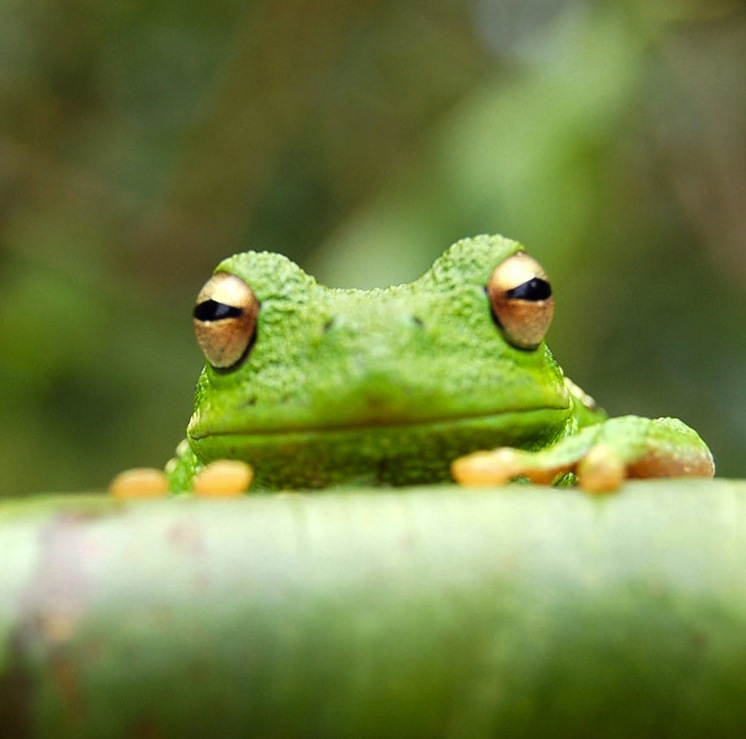
\includegraphics[width=0.1\linewidth]{frog.jpg}
\caption{\label{fig:frog}This frog was uploaded via the file-tree menu.}
\end{figure}


\begin{figure}[ht]
\centering
\begin{subfigure}[b]{0.4\linewidth}
    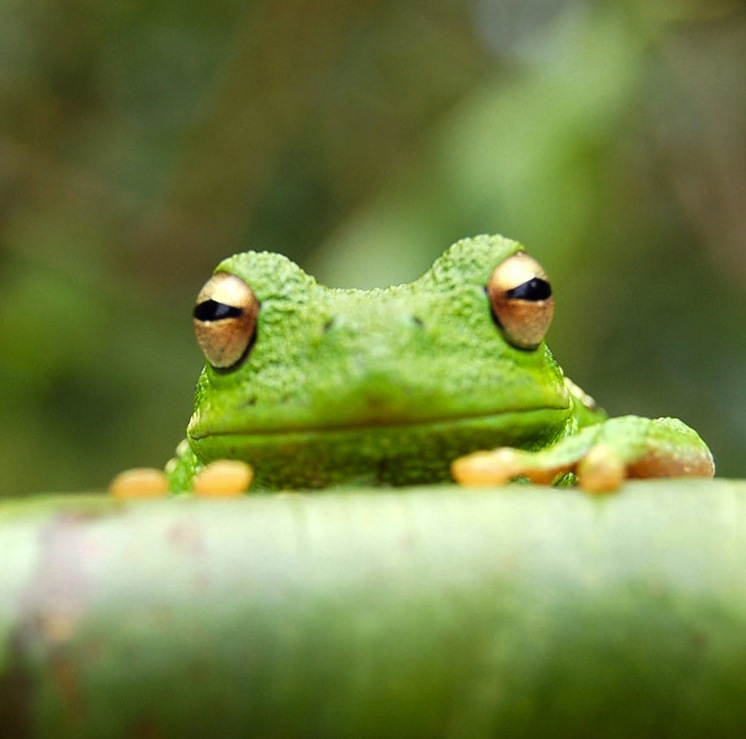
\includegraphics[width=\linewidth]{frog.jpg}
    \caption{}
    \label{subfig:frog1a}
\end{subfigure}
\hspace{0.033\linewidth}
\begin{subfigure}[b]{0.4\linewidth}
    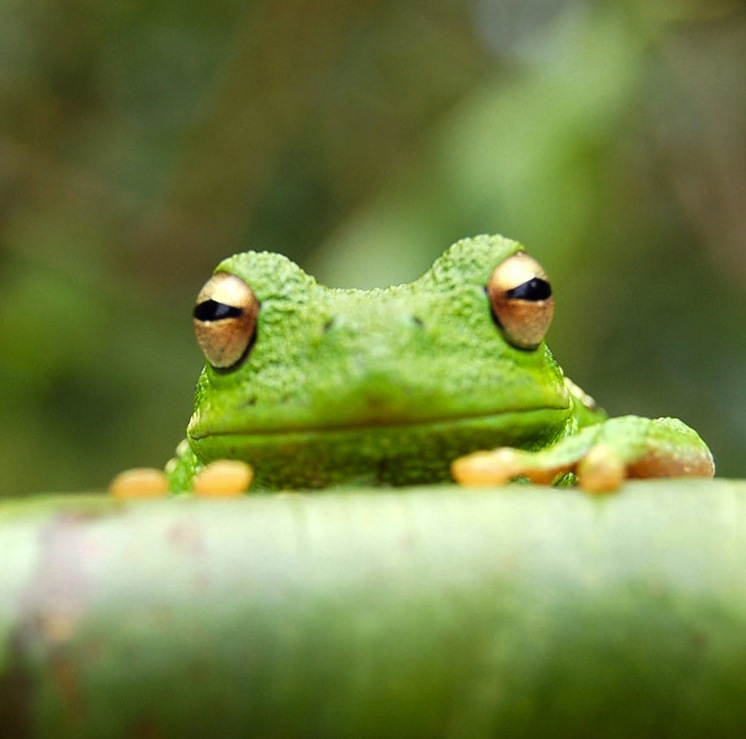
\includegraphics[width=\linewidth]{frog.jpg}
    \caption{}
    \label{subfig:frog1b}
\end{subfigure}
\caption{\textbf{\subref{subfig:frog1a}} This frog was uploaded via the file-tree menu. \textbf{\subref{subfig:frog1b}} So was this. }
\label{fig:frog_ab}
\end{figure}




\begin{figure}[ht]
\centering
\begin{subfigure}[b]{0.75\linewidth}
    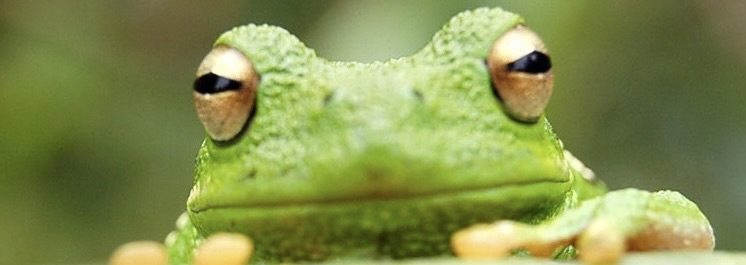
\includegraphics[width=\linewidth]{frog2.jpg}
    \caption{}
    \label{subfig:frog2a}
\end{subfigure}

\begin{subfigure}[b]{0.75\linewidth}
    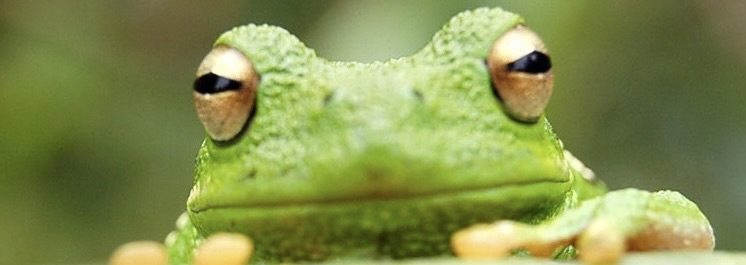
\includegraphics[width=\linewidth]{frog2.jpg}
    \caption{}
    \label{subfig:frog2b}
\end{subfigure}
\caption{\textbf{\subref{subfig:frog2a}} This frog was uploaded via the file-tree menu. \textbf{\subref{subfig:frog2b}} So was this. }
\label{fig:frog_a_b}
\end{figure}



\begin{figure}[ht]
\centering
\begin{subfigure}[b]{0.1\linewidth}
    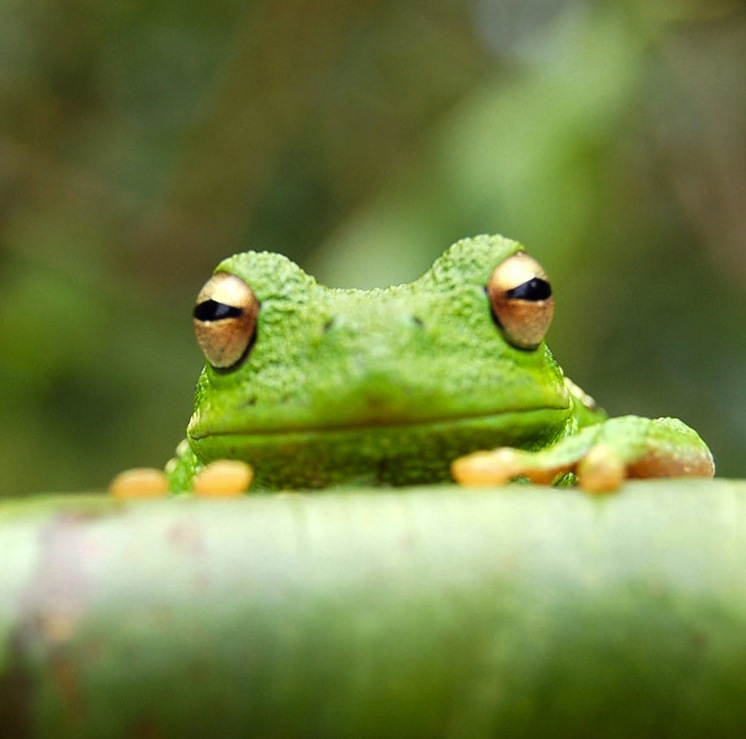
\includegraphics[width=\linewidth]{frog.jpg}
    \caption{}
    \label{subfig:frog3a}
\end{subfigure}
\begin{subfigure}[b]{0.1\linewidth}
    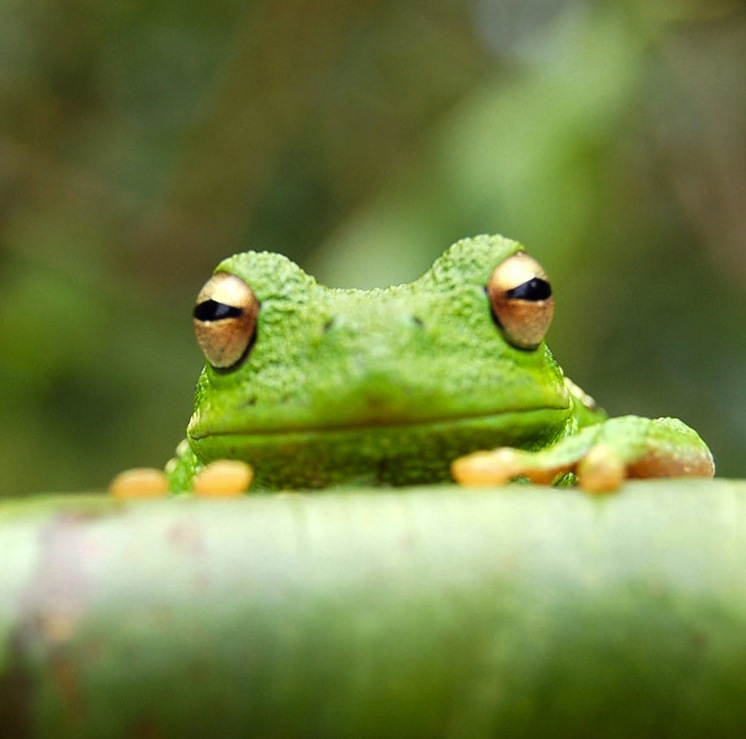
\includegraphics[width=\linewidth]{frog.jpg}
    \caption{}
    \label{subfig:frog3b}
\end{subfigure}
\begin{subfigure}[b]{0.1\linewidth}
    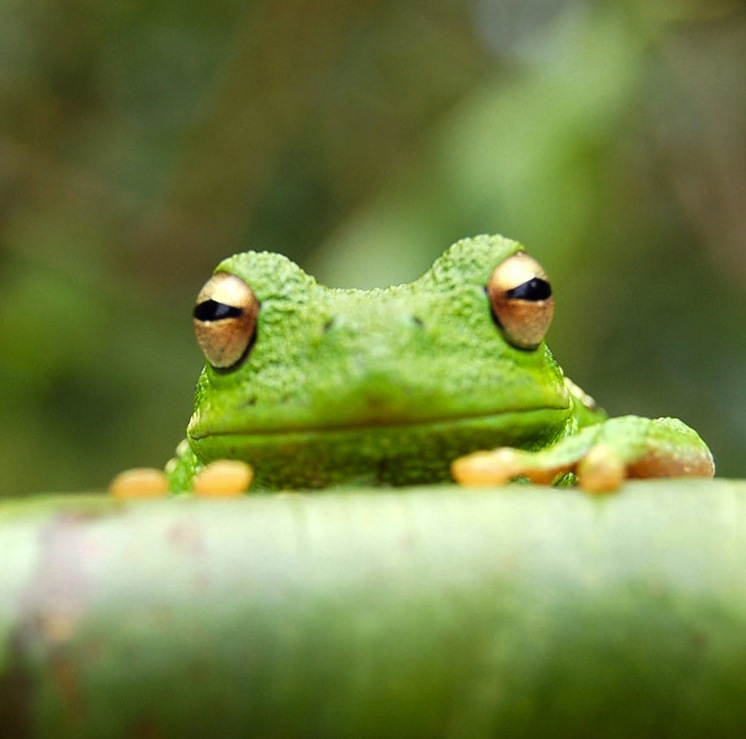
\includegraphics[width=\linewidth]{frog.jpg}
    \caption{}
    \label{subfig:frog3c}
\end{subfigure}
\begin{subfigure}[b]{0.1\linewidth}
    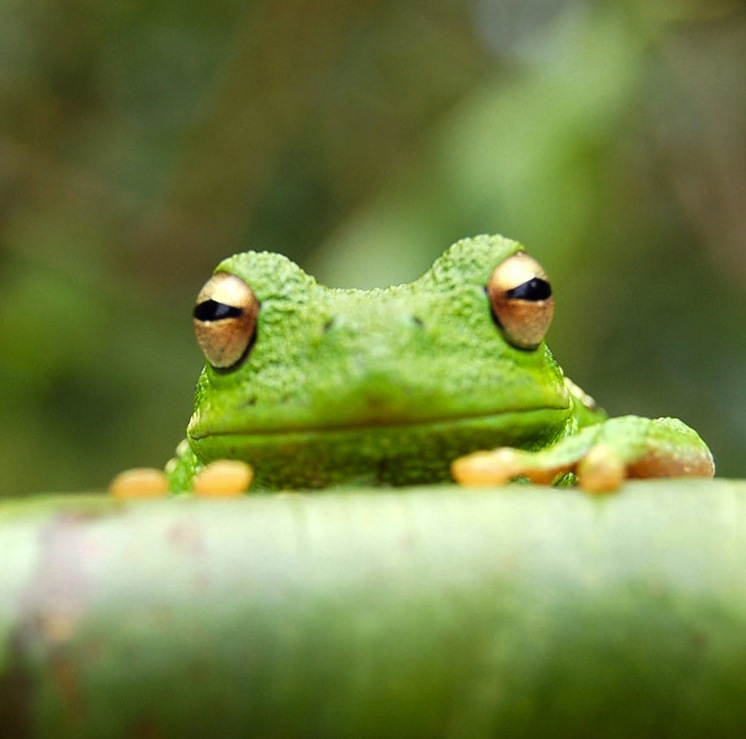
\includegraphics[width=\linewidth]{frog.jpg}
    \caption{}
    \label{subfig:frog3d}
\end{subfigure}
\begin{subfigure}[b]{0.1\linewidth}
    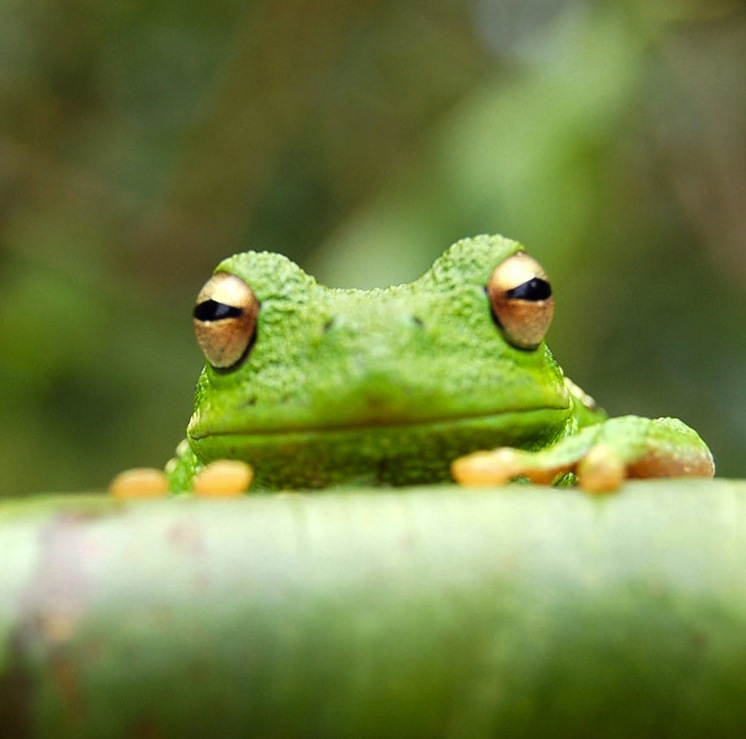
\includegraphics[width=\linewidth]{frog.jpg}
    \caption{}
    \label{subfig:frog3e}
\end{subfigure}
\begin{subfigure}[b]{0.1\linewidth}
    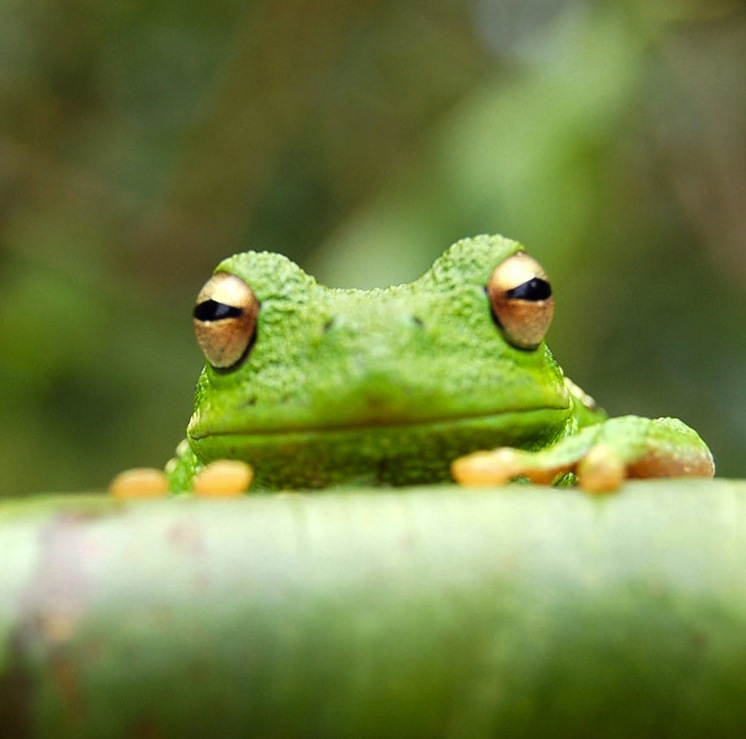
\includegraphics[width=\linewidth]{frog.jpg}
    \caption{}
    \label{subfig:frog3f}
\end{subfigure}
\begin{subfigure}[b]{0.1\linewidth}
    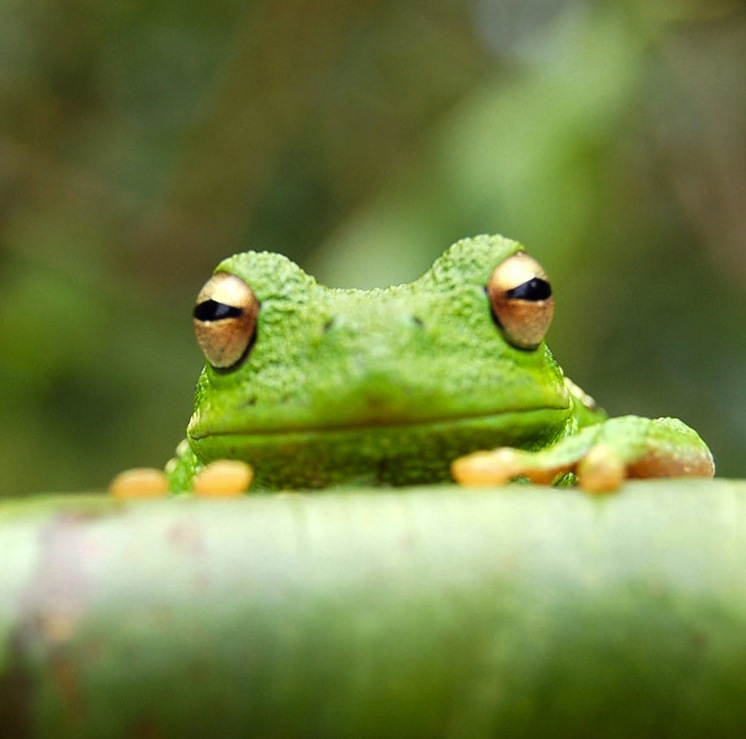
\includegraphics[width=\linewidth]{frog.jpg}
    \caption{}
    \label{subfig:frog3g}
\end{subfigure}
\begin{subfigure}[b]{0.1\linewidth}
    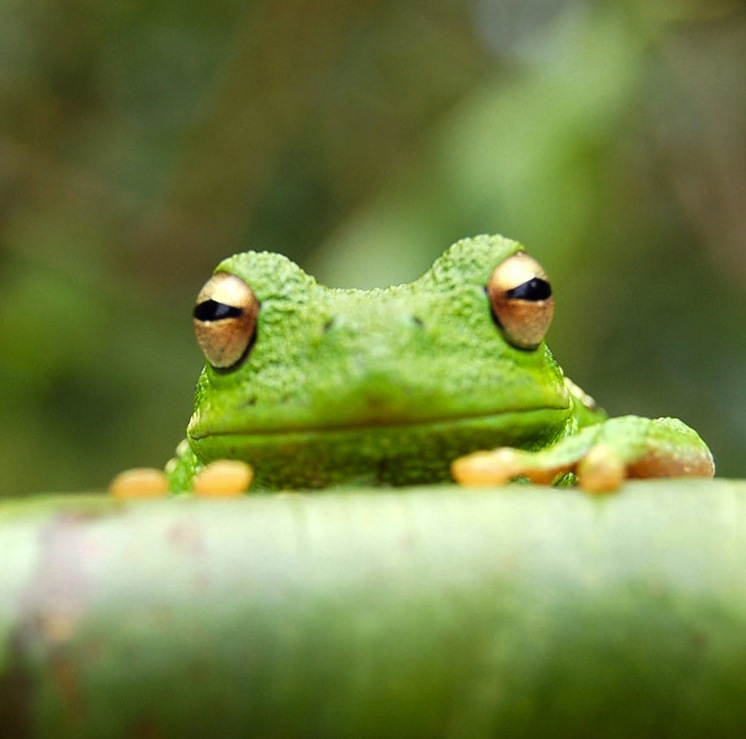
\includegraphics[width=\linewidth]{frog.jpg}
    \caption{}
    \label{subfig:frog3h}
\end{subfigure}
\begin{subfigure}[b]{0.1\linewidth}
    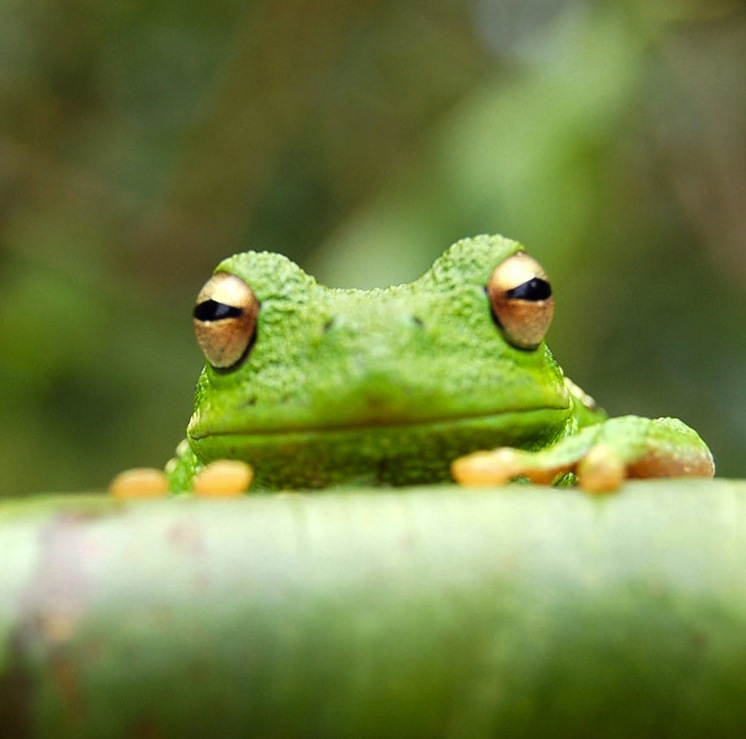
\includegraphics[width=\linewidth]{frog.jpg}
    \caption{}
    \label{subfig:frog3i}
\end{subfigure}

\begin{subfigure}[b]{0.1\linewidth}
    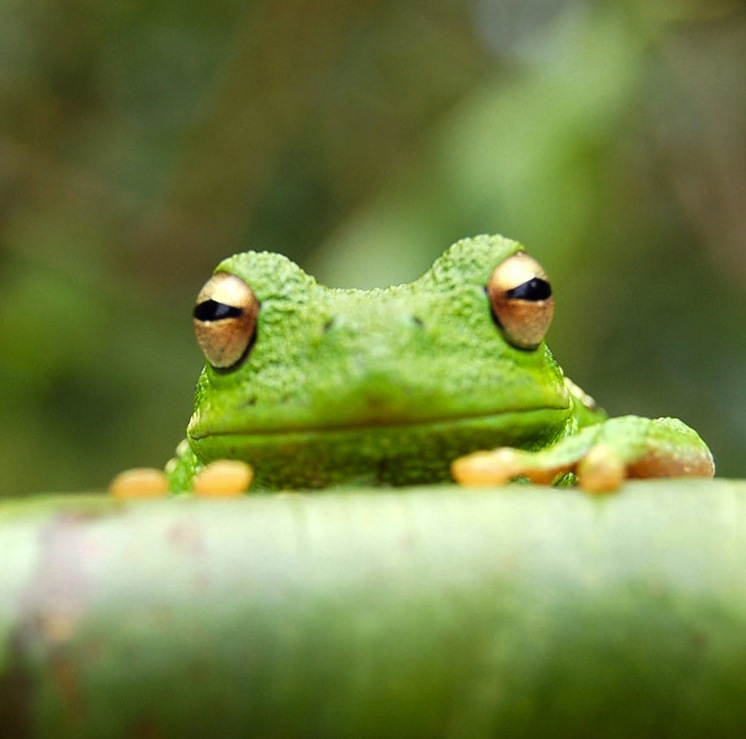
\includegraphics[width=\linewidth]{frog.jpg}
    \caption{}
    \label{subfig:frog3j}
\end{subfigure}
\begin{subfigure}[b]{0.1\linewidth}
    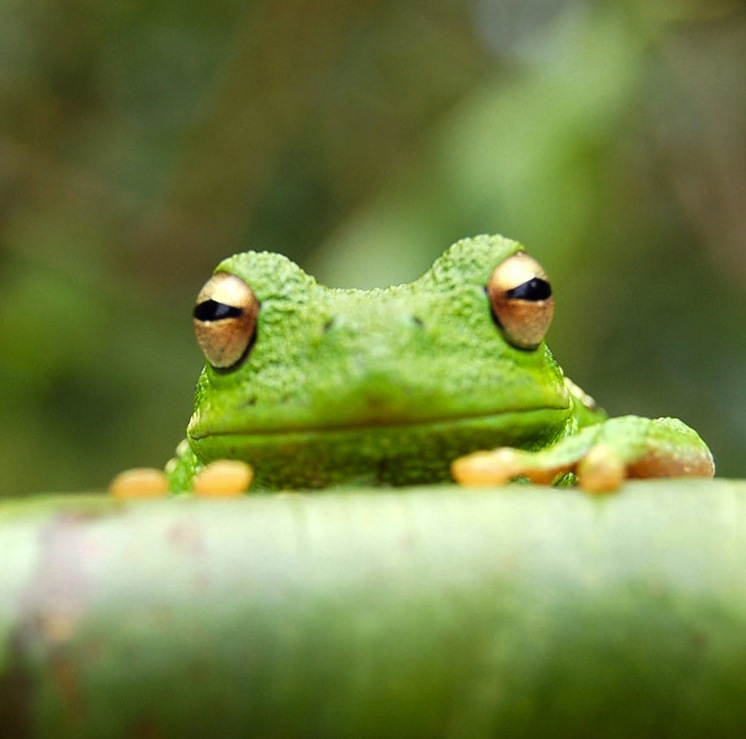
\includegraphics[width=\linewidth]{frog.jpg}
    \caption{}
    \label{subfig:frog3k}
\end{subfigure}
\begin{subfigure}[b]{0.1\linewidth}
    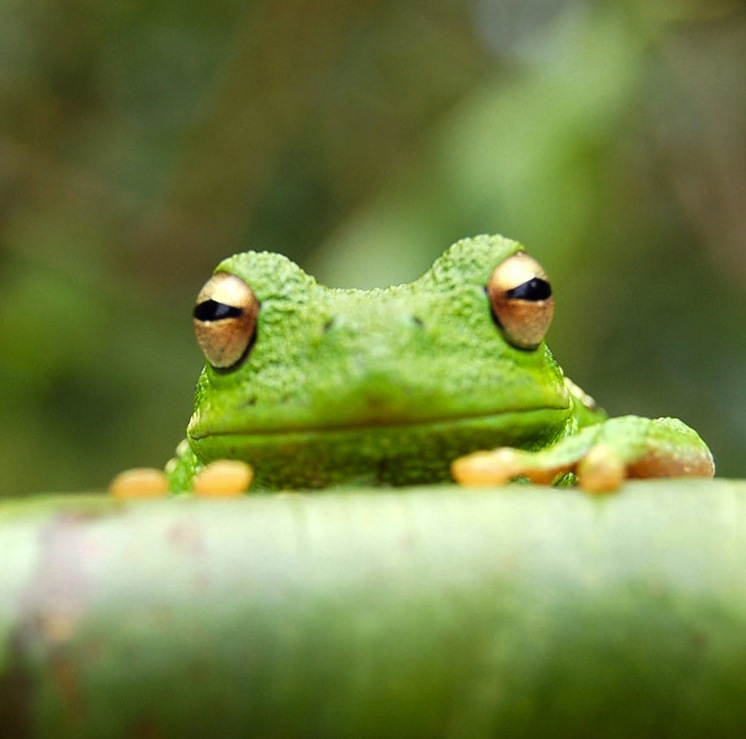
\includegraphics[width=\linewidth]{frog.jpg}
    \caption{}
    \label{subfig:frog3l}
\end{subfigure}
\begin{subfigure}[b]{0.1\linewidth}
    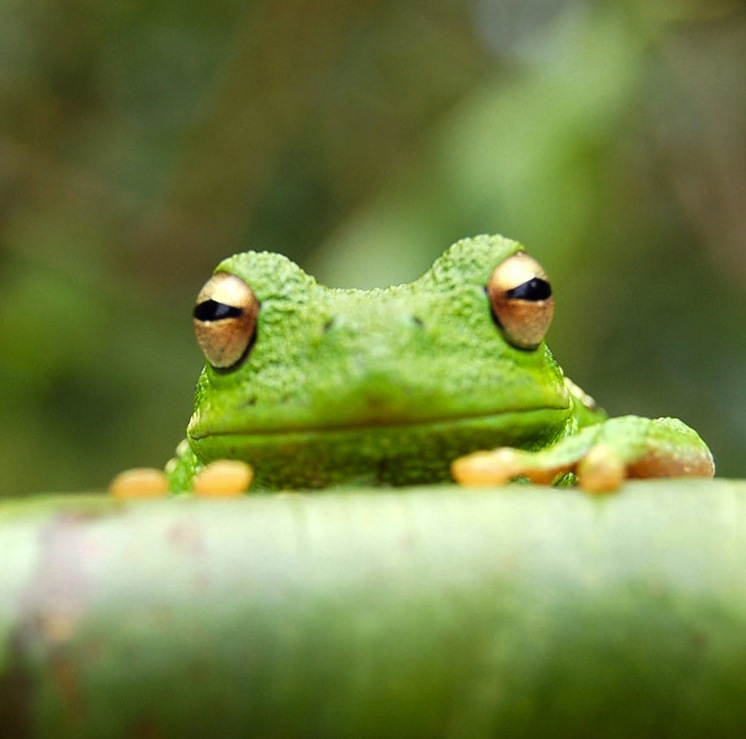
\includegraphics[width=\linewidth]{frog.jpg}
    \caption{}
    \label{subfig:frog3m}
\end{subfigure}
\begin{subfigure}[b]{0.1\linewidth}
    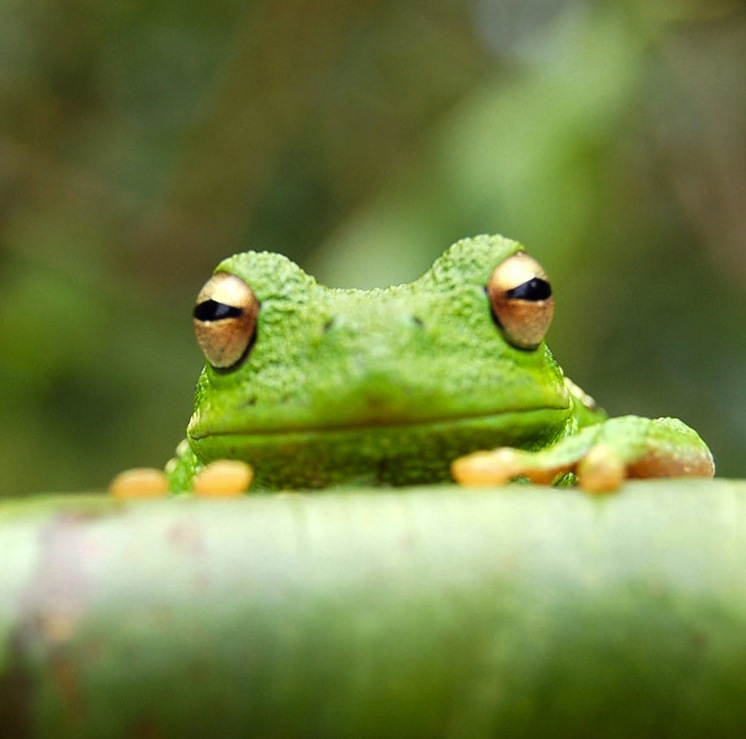
\includegraphics[width=\linewidth]{frog.jpg}
    \caption{}
    \label{subfig:frog3n}
\end{subfigure}
\begin{subfigure}[b]{0.1\linewidth}
    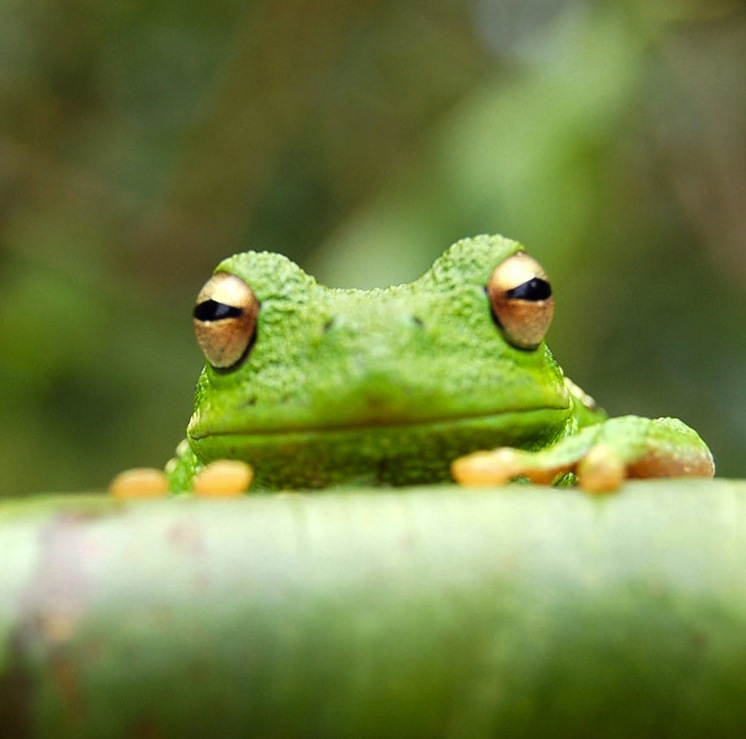
\includegraphics[width=\linewidth]{frog.jpg}
    \caption{}
    \label{subfig:frog3o}
\end{subfigure}
\begin{subfigure}[b]{0.1\linewidth}
    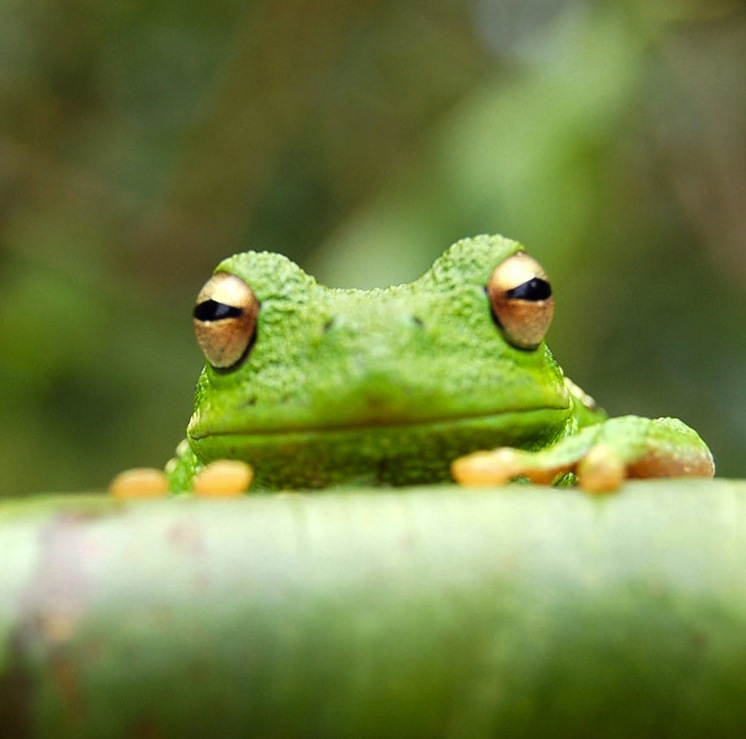
\includegraphics[width=\linewidth]{frog.jpg}
    \caption{}
    \label{subfig:frog3p}
\end{subfigure}
\begin{subfigure}[b]{0.1\linewidth}
    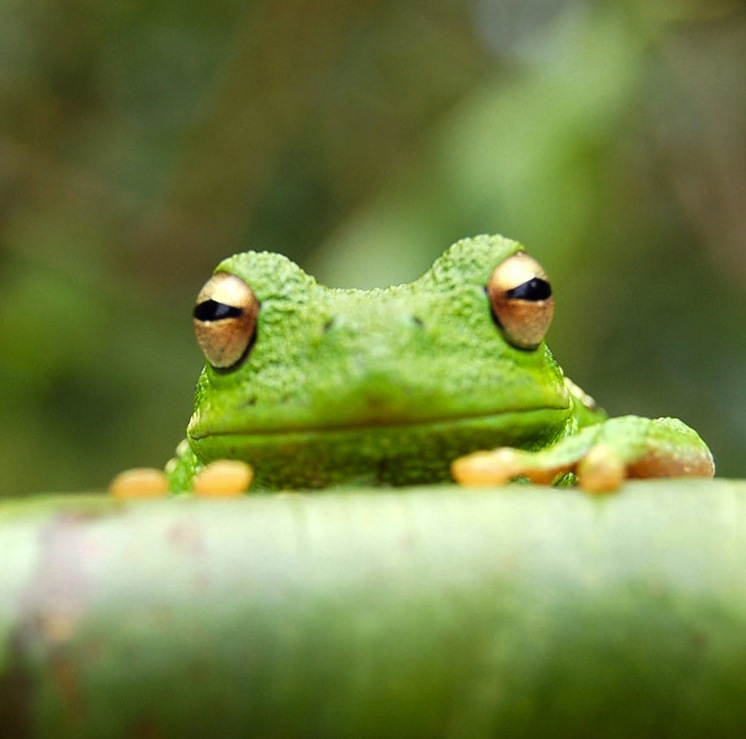
\includegraphics[width=\linewidth]{frog.jpg}
    \caption{}
    \label{subfig:frog3q}
\end{subfigure}
\begin{subfigure}[b]{0.1\linewidth}
    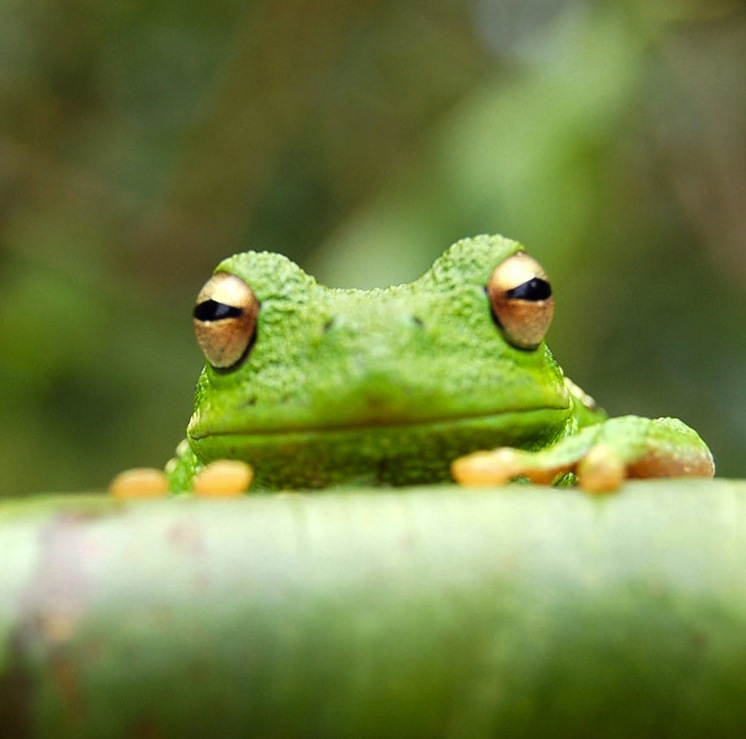
\includegraphics[width=\linewidth]{frog.jpg}
    \caption{}
    \label{subfig:frog3r}
\end{subfigure}
\caption{Here are so many frogs that I won't reference each one in the caption.}
\label{fig:frog_20}
\end{figure}



\begin{figure*}[ht]
\centering
\begin{subfigure}[b]{0.1\linewidth}
    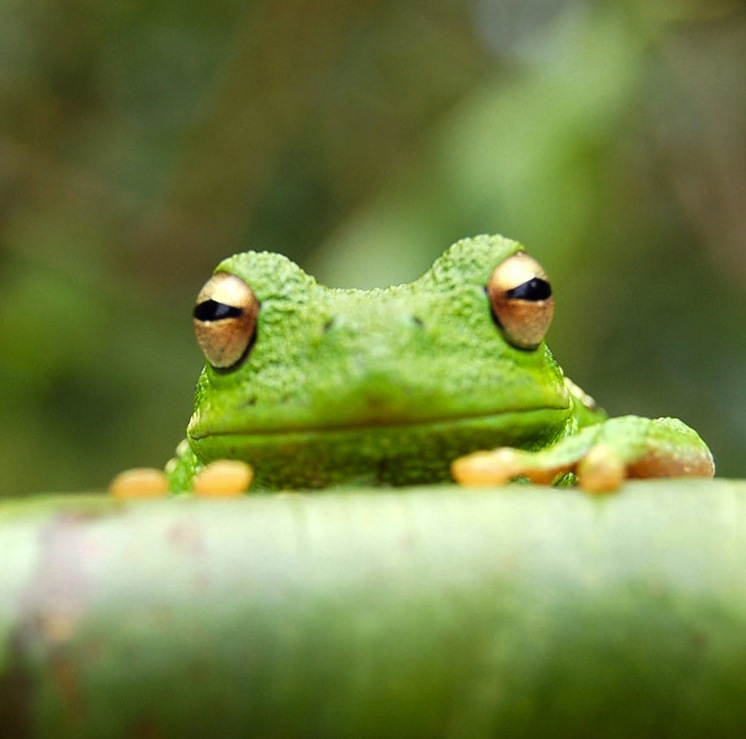
\includegraphics[width=\linewidth]{frog.jpg}
    \caption{}
    \label{subfig:frog4a}
\end{subfigure}
\begin{subfigure}[b]{0.1\linewidth}
    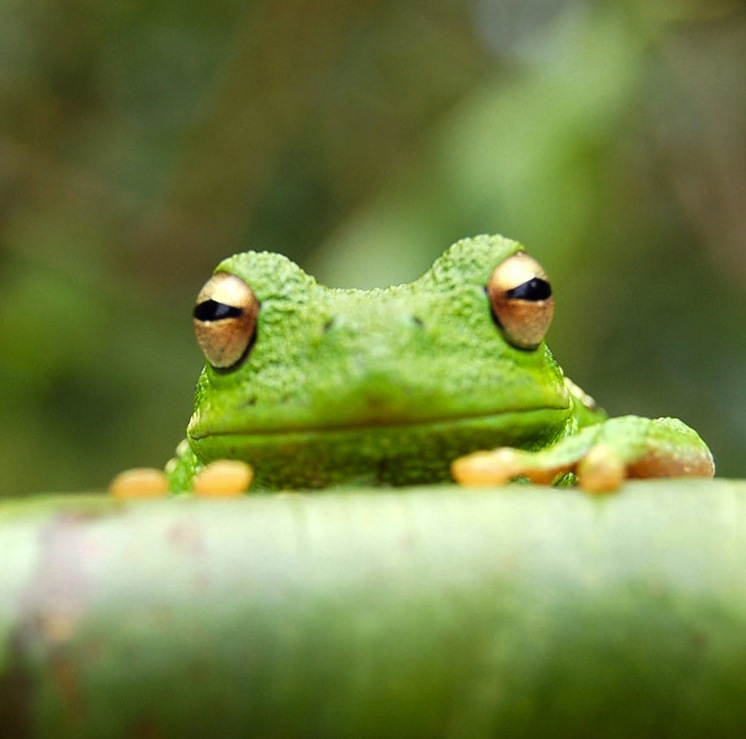
\includegraphics[width=\linewidth]{frog.jpg}
    \caption{}
    \label{subfig:frog4b}
\end{subfigure}
\begin{subfigure}[b]{0.1\linewidth}
    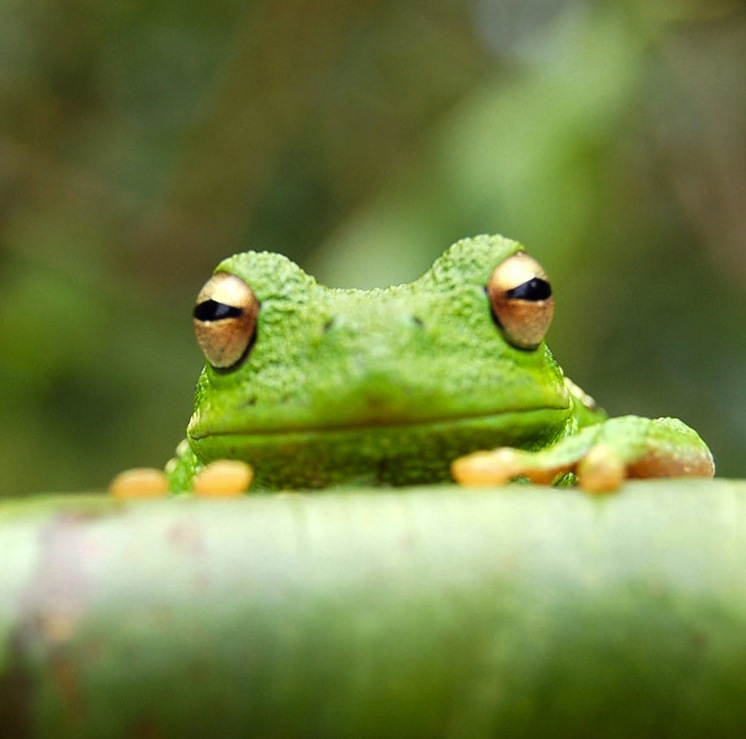
\includegraphics[width=\linewidth]{frog.jpg}
    \caption{}
    \label{subfig:frog4c}
\end{subfigure}
\begin{subfigure}[b]{0.1\linewidth}
    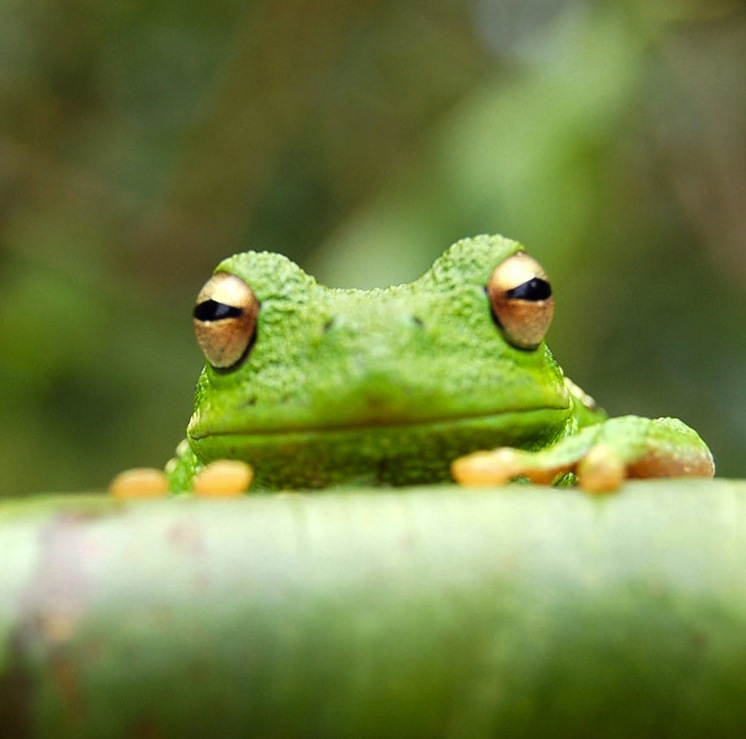
\includegraphics[width=\linewidth]{frog.jpg}
    \caption{}
    \label{subfig:frog4d}
\end{subfigure}
\begin{subfigure}[b]{0.1\linewidth}
    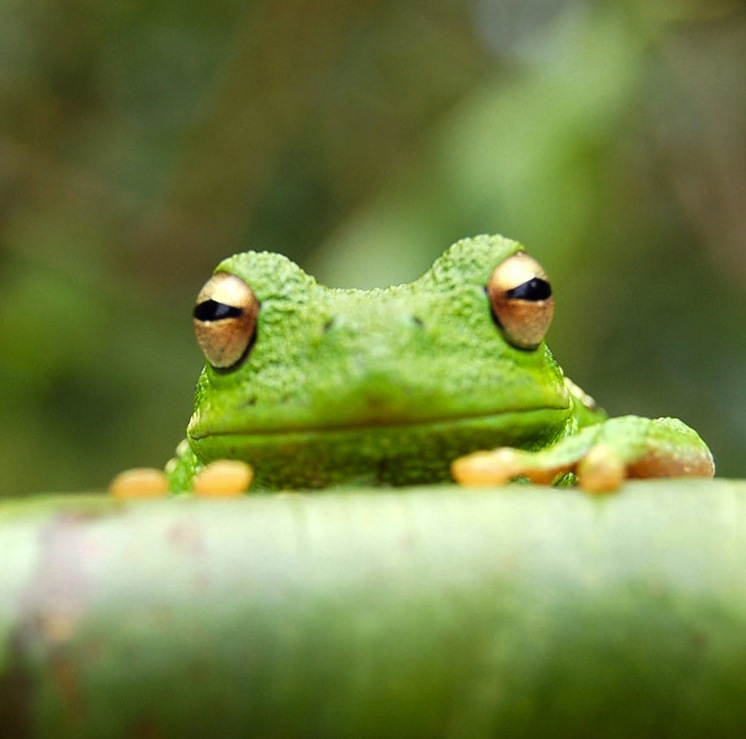
\includegraphics[width=\linewidth]{frog.jpg}
    \caption{}
    \label{subfig:frog4e}
\end{subfigure}
\begin{subfigure}[b]{0.1\linewidth}
    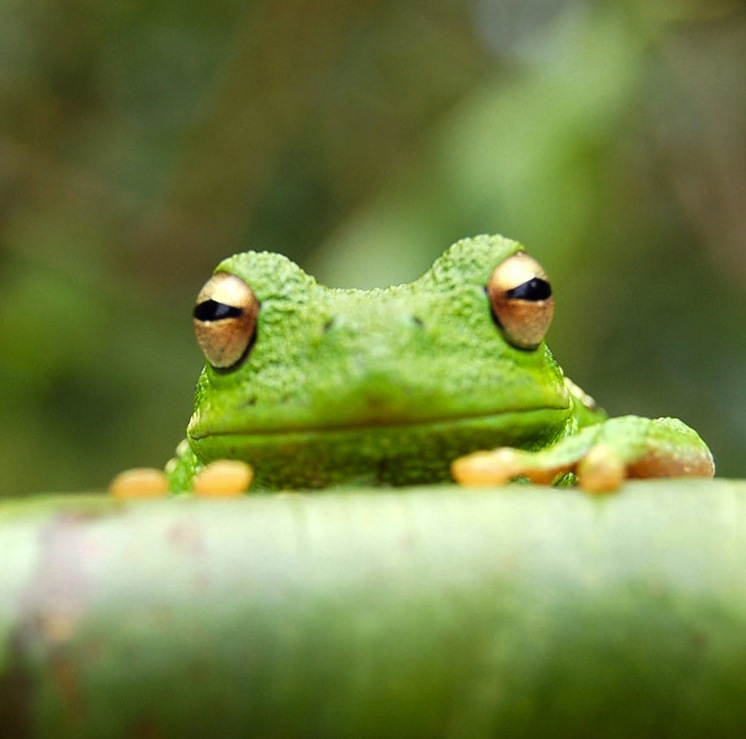
\includegraphics[width=\linewidth]{frog.jpg}
    \caption{}
    \label{subfig:frog4f}
\end{subfigure}
\begin{subfigure}[b]{0.1\linewidth}
    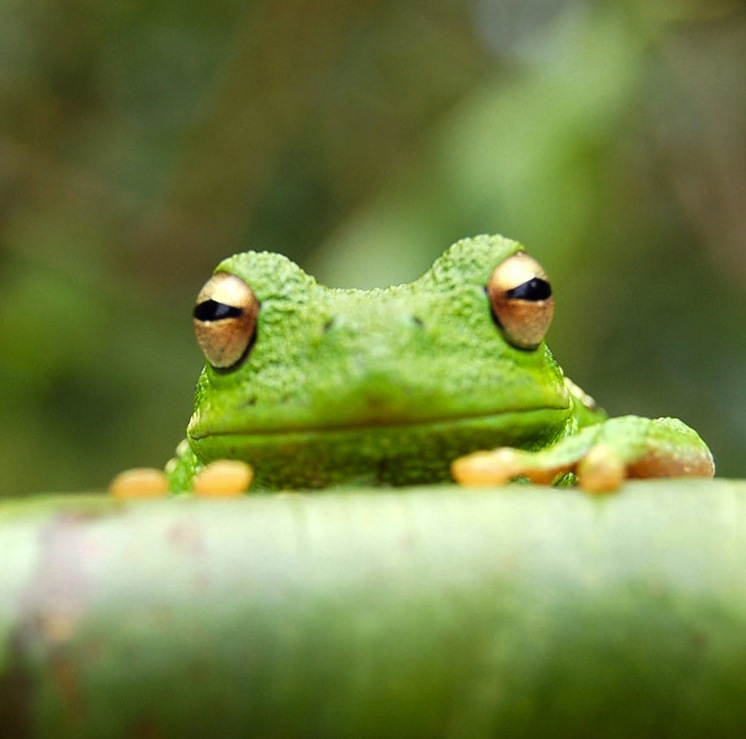
\includegraphics[width=\linewidth]{frog.jpg}
    \caption{}
    \label{subfig:frog4g}
\end{subfigure}
\begin{subfigure}[b]{0.1\linewidth}
    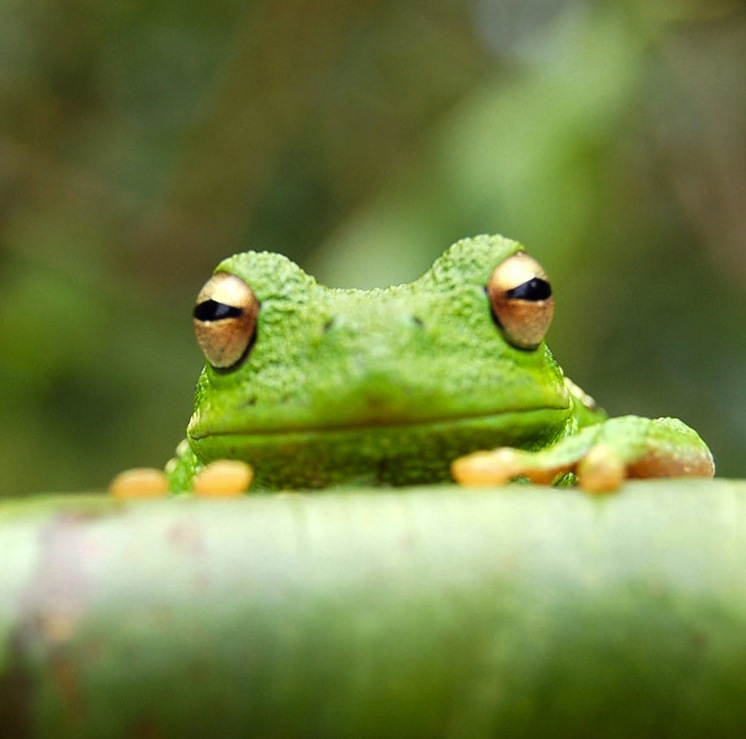
\includegraphics[width=\linewidth]{frog.jpg}
    \caption{}
    \label{subfig:frog4h}
\end{subfigure}
\begin{subfigure}[b]{0.1\linewidth}
    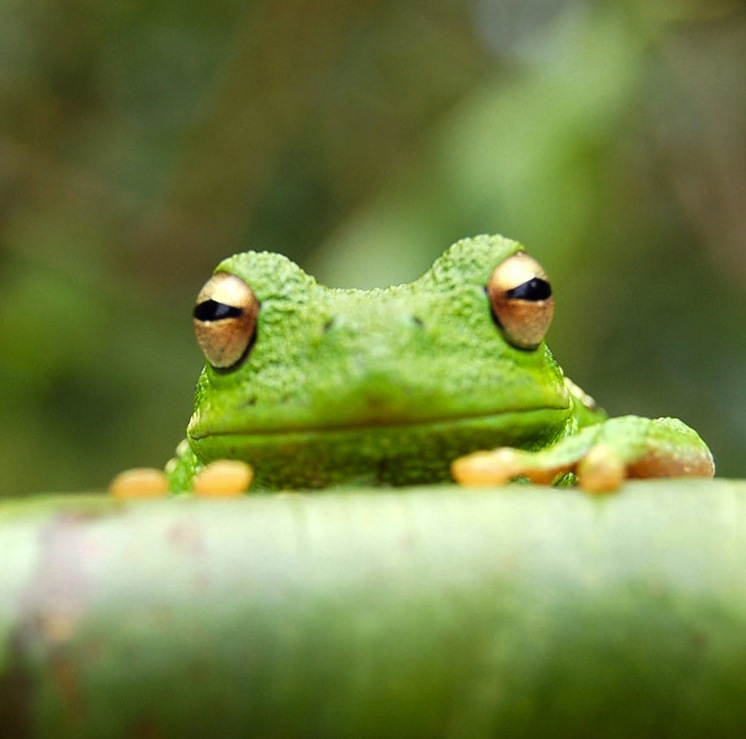
\includegraphics[width=\linewidth]{frog.jpg}
    \caption{}
    \label{subfig:frog4i}
\end{subfigure}

\begin{subfigure}[b]{0.1\linewidth}
    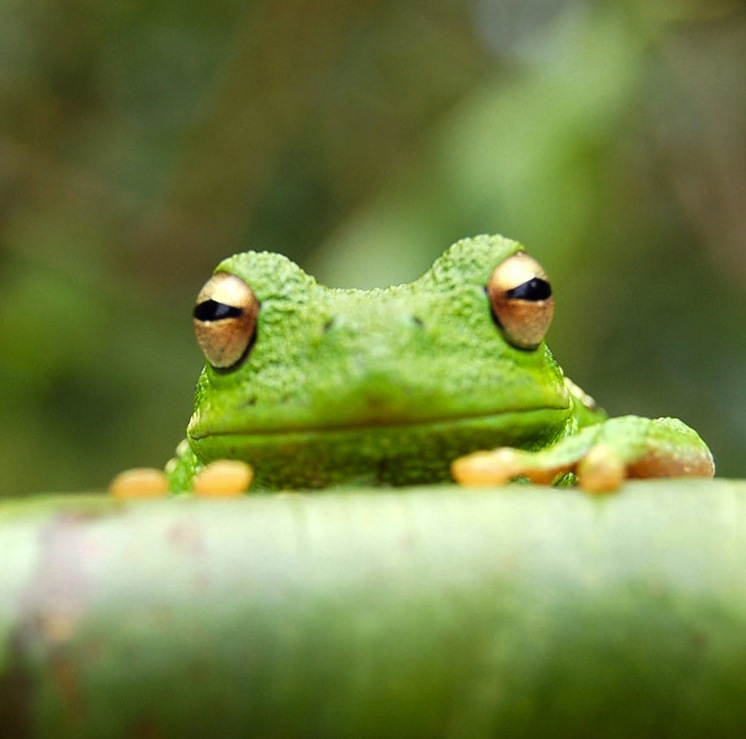
\includegraphics[width=\linewidth]{frog.jpg}
    \caption{}
    \label{subfig:frog4j}
\end{subfigure}
\begin{subfigure}[b]{0.1\linewidth}
    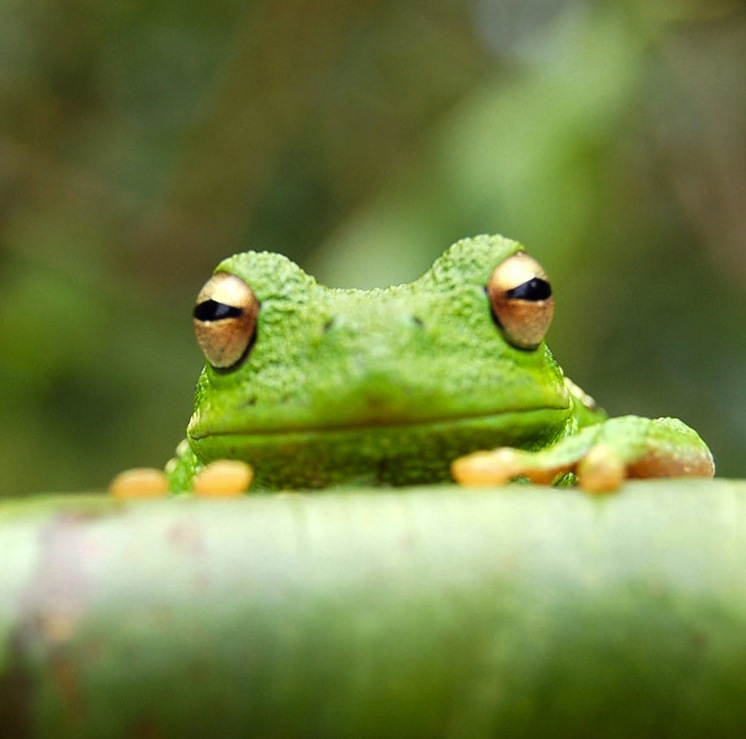
\includegraphics[width=\linewidth]{frog.jpg}
    \caption{}
    \label{subfig:frog4k}
\end{subfigure}
\begin{subfigure}[b]{0.1\linewidth}
    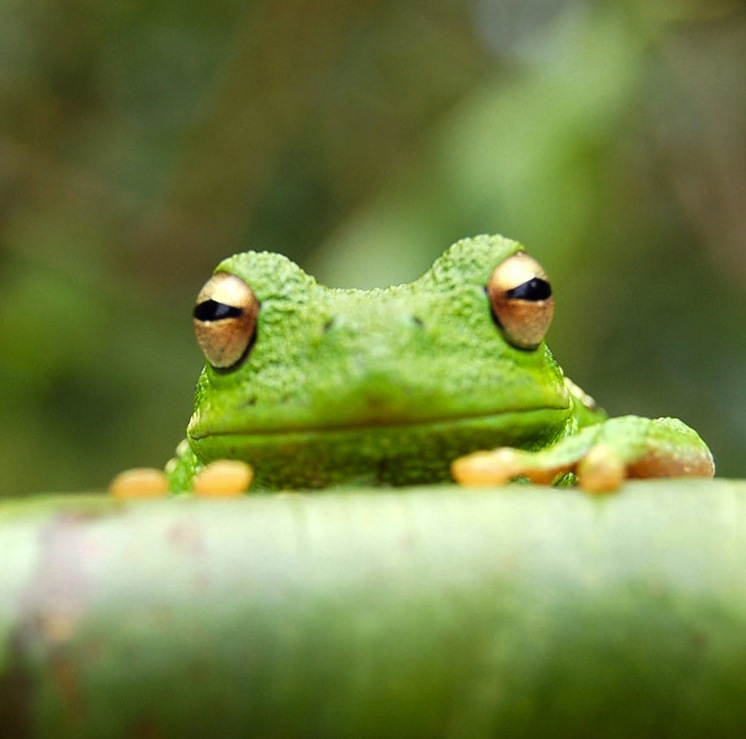
\includegraphics[width=\linewidth]{frog.jpg}
    \caption{}
    \label{subfig:frog4l}
\end{subfigure}
\begin{subfigure}[b]{0.1\linewidth}
    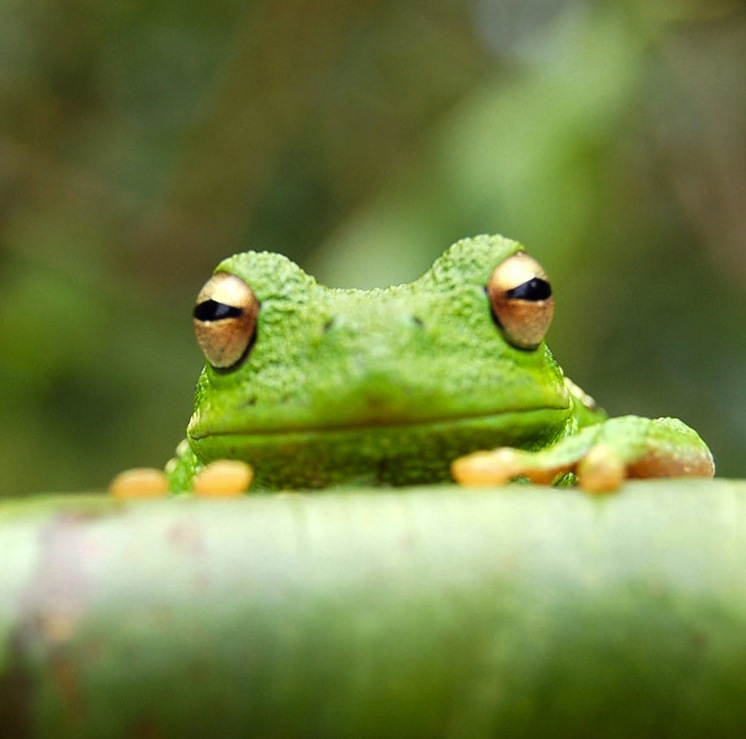
\includegraphics[width=\linewidth]{frog.jpg}
    \caption{}
    \label{subfig:frog4m}
\end{subfigure}
\begin{subfigure}[b]{0.1\linewidth}
    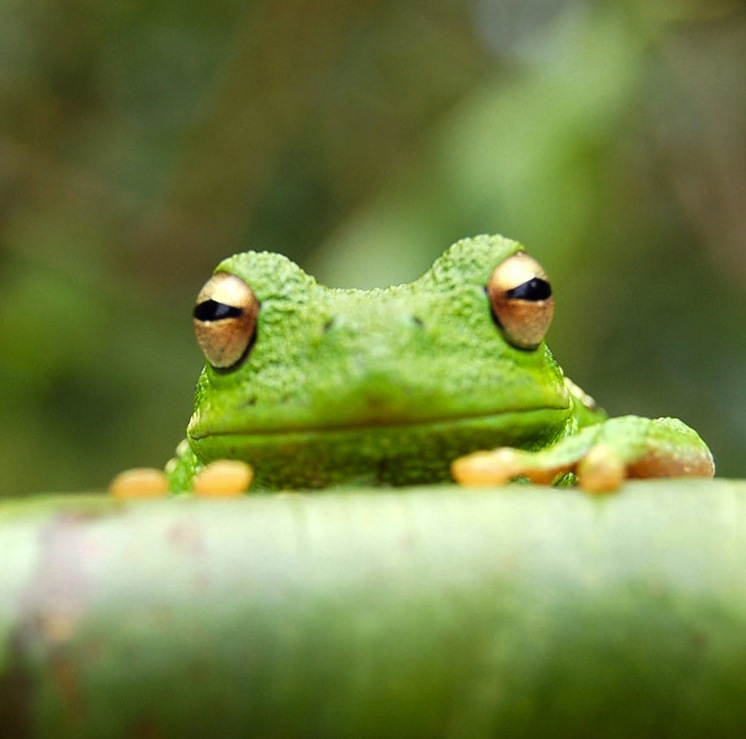
\includegraphics[width=\linewidth]{frog.jpg}
    \caption{}
    \label{subfig:frog4n}
\end{subfigure}
\begin{subfigure}[b]{0.1\linewidth}
    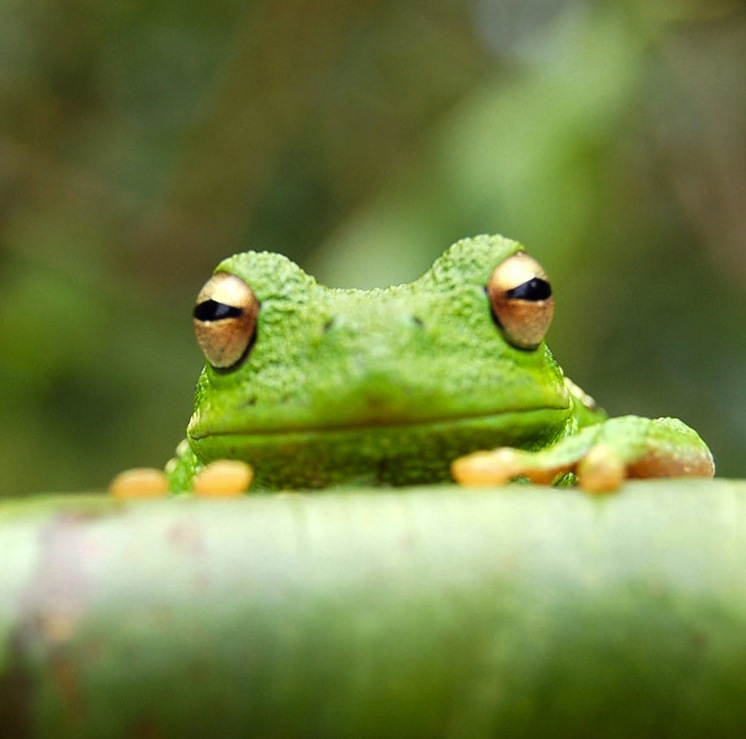
\includegraphics[width=\linewidth]{frog.jpg}
    \caption{}
    \label{subfig:frog4o}
\end{subfigure}
\begin{subfigure}[b]{0.1\linewidth}
    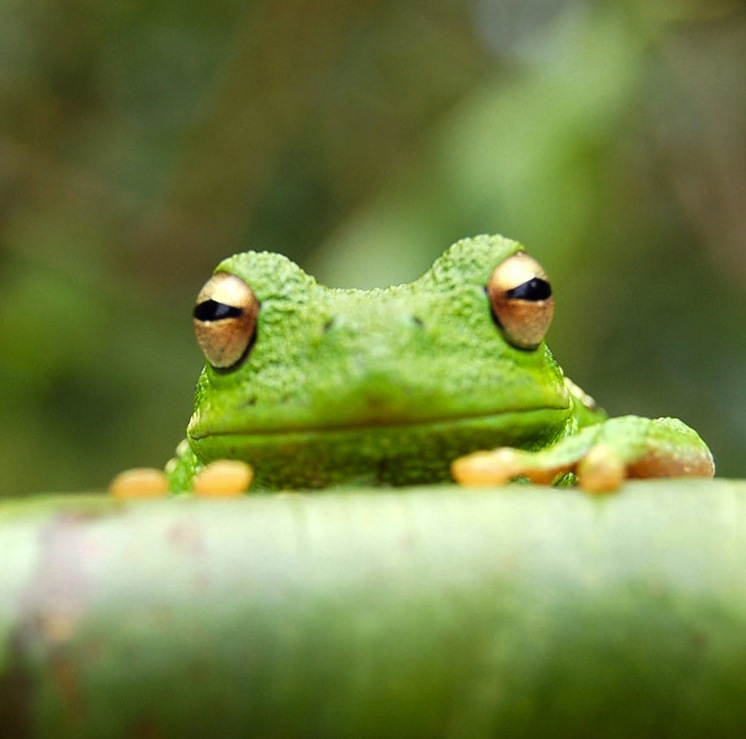
\includegraphics[width=\linewidth]{frog.jpg}
    \caption{}
    \label{subfig:frog4p}
\end{subfigure}
\begin{subfigure}[b]{0.1\linewidth}
    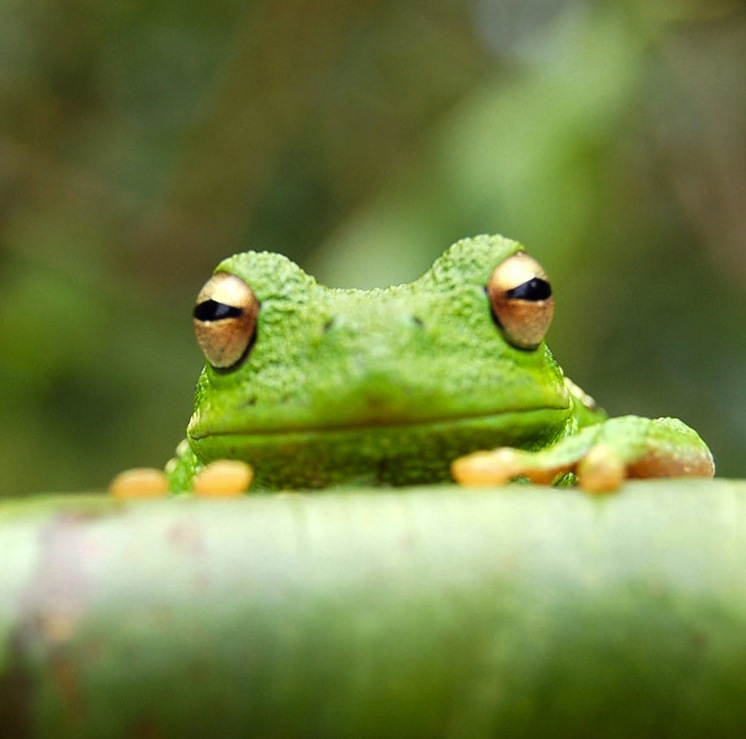
\includegraphics[width=\linewidth]{frog.jpg}
    \caption{}
    \label{subfig:frog4q}
\end{subfigure}
\begin{subfigure}[b]{0.1\linewidth}
    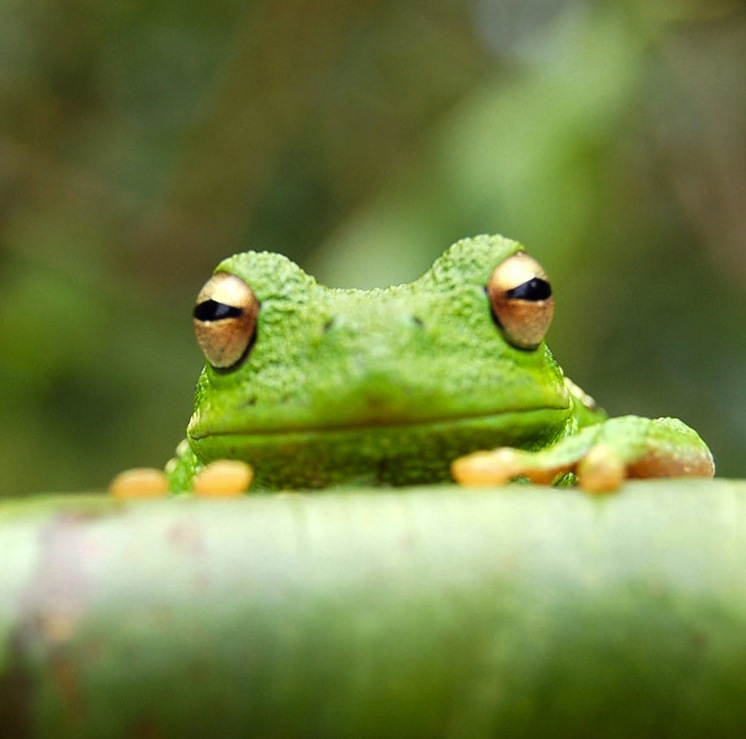
\includegraphics[width=\linewidth]{frog.jpg}
    \caption{}
    \label{subfig:frog4r}
\end{subfigure}
\caption{And I'm doing this across columns too...}
\label{fig:frog_20_span}
\end{figure*}



You can also add double column figures by using \textbackslash begin\{figure*\}


\begin{figure*}[ht]
\centering
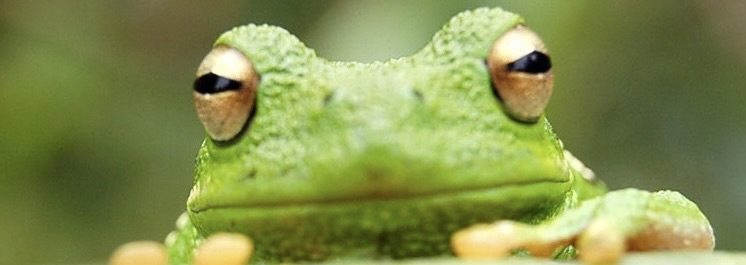
\includegraphics[width=0.9\linewidth]{frog2.jpg}
\caption{\label{fig:frog2}This frog was uploaded via the file-tree menu.}
\end{figure*}

\subsection{How to add Tables}

Use the table and tabular environments for basic tables --- see Table~\ref{tab:widgets} and ~\ref{tab:widgets_wide}, for example. For more information, please see this help article on \href{https://www.overleaf.com/learn/latex/tables}{tables}. 

\begin{table}[ht]
\centering
\begin{tabular}{l|r|r|r|r|r|r|r|r|r|r|r|r|r}
Item & Quantity & other & other & other & other  \\\hline
Widgets & 42 & thing & thing & thing & thing  \\
Gadgets & 13 & thing & thing & thing & thing 
\end{tabular}
\caption{\label{tab:widgets}An example spanning columns table.}
\end{table}



\begin{table*}[ht]
\centering
\begin{tabular}{l|r|r|r|r|r|r|r|r|r|r|r|r|r}
Item & Quantity & other & other & other & other & other & other & other & other  & other & other & other & other  \\\hline
Widgets & 42 & thing & thing & thing & thing & thing & thing & thing & thing & thing & thing & thing & thing \\
Gadgets & 13 & thing & thing & thing & thing & thing & thing & thing & thing & thing & thing & thing & thing
\end{tabular}
\caption{\label{tab:widgets_wide}An example spanning columns table.}
\end{table*}

\subsection{How to add Comments and Track Changes}

Comments can be added to your project by highlighting some text and clicking ``Add comment'' in the top right of the editor pane. To view existing comments, click on the Review menu in the toolbar above. To reply to a comment, click on the Reply button in the lower right corner of the comment. You can close the Review pane by clicking its name on the toolbar when you're done reviewing for the time being.

Track changes are available on all our \href{https://www.overleaf.com/user/subscription/plans}{premium plans}, and can be toggled on or off using the option at the top of the Review pane. Track changes allow you to keep track of every change made to the document, along with the person making the change. 

\subsection{How to add Lists}

You can make lists with automatic numbering \dots

\begin{enumerate}
\item Like this,
\item and like this.
\end{enumerate}
\dots or bullet points \dots
\begin{itemize}
\item Like this,
\item and like this.
\end{itemize}

\subsection{How to write Mathematics}

\LaTeX{} is great at typesetting mathematics. Let $X_1, X_2, \ldots, X_n$ be a sequence of independent and identically distributed random variables with $\text{E}[X_i] = \mu$ and $\text{Var}[X_i] = \sigma^2 < \infty$, and let
\[S_n = \frac{X_1 + X_2 + \cdots + X_n}{n}
      = \frac{1}{n}\sum_{i}^{n} X_i\]
denote their mean. Then as $n$ approaches infinity, the random variables $\sqrt{n}(S_n - \mu)$ converge in distribution to a normal $\mathcal{N}(0, \sigma^2)$.


\subsection{How to change the margins and paper size}

Usually the template you're using will have the page margins and paper size set correctly for that use-case. For example, if you're using a journal article template provided by the journal publisher, that template will be formatted according to their requirements. In these cases, it's best not to alter the margins directly.

If however you're using a more general template, such as this one, and would like to alter the margins, a common way to do so is via the geometry package. You can find the geometry package loaded in the preamble at the top of this example file, and if you'd like to learn more about how to adjust the settings, please visit this help article on \href{https://www.overleaf.com/learn/latex/page_size_and_margins}{page size and margins}.

\subsection{How to change the document language and spell check settings}

Overleaf supports many different languages, including multiple different languages within one document. 

To configure the document language, simply edit the option provided to the babel package in the preamble at the top of this example project. To learn more about the different options, please visit this help article on \href{https://www.overleaf.com/learn/latex/International_language_support}{international language support}.

To change the spell check language, simply open the Overleaf menu at the top left of the editor window, scroll down to the spell check setting, and adjust accordingly.

\subsection{How to add Citations and a References List}

You can simply upload a \verb|.bib| file containing your BibTeX entries, created with a tool such as JabRef. You can then cite entries from it, like this \cite{greenwade93}. Just remember to specify a bibliography style, as well as the filename of the \verb|.bib|. You can find a \href{https://www.overleaf.com/help/97-how-to-include-a-bibliography-using-bibtex}{video tutorial here} to learn more about BibTeX.

If you have an \href{https://www.overleaf.com/user/subscription/plans}{upgraded account}, you can also import your Mendeley or Zotero library directly as a \verb|.bib| file, via the upload menu in the file-tree.

\subsection{Good luck!}

We hope you find Overleaf useful, and do take a look at our \href{https://www.overleaf.com/learn}{help library} for more tutorials and user guides! Please also let us know if you have any feedback using the Contact Us link at the bottom of the Overleaf menu --- or use the contact form at \url{https://www.overleaf.com/contact}.


\subsection{A bunch of text from ChatGPT to fill out the next page}

This text was produced by ChatGPT, visualised in Figure \ref{fig:chatgpt}.



\begin{figure}[ht]
\centering

\includegraphics[width=0.99\linewidth]{AI.jpeg}
\caption{\label{fig:chatgpt}This is ChatGPT personified!}
\end{figure}

\subsubsection{LaTeX}

LaTeX, pronounced "Lay-tech" or "Lah-tech," is a powerful and versatile typesetting system used for creating beautifully formatted documents. Its strengths lie in several aspects, making it a favorite among users worldwide.

Firstly, one of the most appealing aspects of LaTeX is its unparalleled typesetting quality. It produces high-quality documents, especially for technical and scientific writing. Whether it's academic papers, theses, reports, or books, LaTeX ensures professional and consistent formatting, including superior handling of mathematical equations, complex symbols, and references.

The system's ability to handle mathematical typesetting is second to none. LaTeX provides a comprehensive suite of tools for rendering intricate mathematical expressions and equations effortlessly. This feature is invaluable for mathematicians, physicists, engineers, and researchers who require precision and clarity in their documents.

Another compelling aspect of LaTeX is its focus on content separation and reusability. Users can separate content from formatting by using markup and style files, allowing them to focus on writing without getting bogged down by design concerns. Additionally, LaTeX enables the creation of templates, making it easy to reuse document structures and styles across various projects.

Moreover, LaTeX is an open-source platform, freely available for anyone to use and modify. This aspect has fostered a vibrant and supportive community of users who contribute packages, templates, and solutions to common issues. The extensive range of packages and extensions available for LaTeX greatly enhances its functionality and flexibility, catering to diverse user needs.

The system's cross-compatibility is another appealing trait. LaTeX documents can be easily converted to various formats like PDF, HTML, and others, ensuring accessibility across different platforms and devices without compromising quality.

Furthermore, LaTeX promotes collaboration and version control. Its plain text format facilitates easy collaboration among multiple authors using version control systems like Git, allowing efficient tracking of changes and contributions.

Despite its numerous advantages, LaTeX does have a learning curve. Its syntax may appear intimidating at first, especially for beginners accustomed to word processors. However, with practice and resources like online tutorials, forums, and documentation, users can quickly grasp the fundamentals and harness the system's capabilities effectively.

In conclusion, LaTeX stands out as a remarkable typesetting system cherished for its exceptional quality, mathematical typesetting capabilities, content separation, community support, open-source nature, cross-compatibility, and facilitation of collaboration. Its influence continues to grow, catering to the needs of diverse users seeking precision, professionalism, and flexibility in document preparation.


\subsubsection{Frogs}

Frogs, members of the amphibian class Anura, are captivating creatures that have fascinated humans for centuries. These remarkable amphibians have carved a niche in ecosystems worldwide, symbolizing both diversity and resilience in the natural world.

Frogs inhabit a wide range of environments, from lush rainforests to arid deserts, and can be found on every continent except Antarctica. Their adaptability allows them to thrive in diverse climates, showcasing an incredible array of species, each with unique characteristics and behaviors.

One of the most striking features of frogs is their life cycle, which undergoes a fascinating transformation known as metamorphosis. Starting as tadpoles—tiny aquatic larvae with gills—frogs develop into adults, undergoing a remarkable change where they grow limbs, lose their tails, and develop lungs for breathing air. This process of transformation symbolizes resilience, adaptability, and the beauty of natural progression.

Frogs play pivotal roles in various ecosystems as both predators and prey. As carnivorous creatures, they contribute to controlling insect populations, helping to maintain ecological balance. Their diet mainly consists of insects, making them an essential component in controlling pest populations, thus benefiting agricultural systems.

Moreover, frogs serve as indicators of environmental health. Their sensitive and permeable skin makes them susceptible to changes in environmental conditions, including pollution, habitat loss, and climate change. Declines in frog populations worldwide serve as alarm bells for broader environmental issues, prompting conservation efforts to protect not only these amphibians but also the ecosystems they inhabit.

These remarkable creatures have also fascinated cultures worldwide, appearing in folklore, mythology, and symbolism. In many cultures, frogs represent transformation, fertility, and good fortune. Their unique life cycle, from water-dwelling tadpoles to land-roaming adults, has been a source of inspiration in various cultural narratives, often symbolizing adaptation and change.

Additionally, frogs contribute significantly to scientific research. Their unique characteristics, such as the ability to breathe through their skin, have made them subjects of scientific inquiry. Studies on frogs have contributed to medical research, particularly in understanding skin permeability, disease resistance, and potential applications in pharmaceuticals.

Frogs also possess an incredible diversity in their vocalizations. Their croaks, chirps, and calls serve various purposes, from attracting mates to establishing territories. This communication through sound is an essential aspect of their behavior and is often a defining feature of nighttime environments in many regions.

Despite their significance and contributions to ecosystems and human culture, frogs face numerous threats. Habitat destruction, pollution, climate change, invasive species, and diseases like chytrid fungus pose significant challenges to their survival. Conservation efforts, including habitat preservation, captive breeding programs, and public awareness campaigns, are crucial for ensuring the survival of these fascinating amphibians.

In conclusion, frogs represent a fascinating aspect of the natural world, embodying resilience, diversity, and ecological significance. Their captivating life cycle, ecological roles, cultural symbolism, scientific importance, and unique vocalizations make them integral components of our ecosystems and cultural heritage. As we navigate environmental challenges, preserving the habitats and protecting the populations of these remarkable creatures becomes increasingly vital for maintaining the biodiversity of our planet.


\bibliographystyle{vancouver}
\bibliography{sample}



\end{document}